%% 
%% Copyright 2007, 2008, 2009 Elsevier Ltd
%% 
%% This file is part of the 'Elsarticle Bundle'.
%% ---------------------------------------------
%% 
%% It may be distributed under the conditions of the LaTeX Project Public
%% License, either version 1.2 of this license or (at your option) any
%% later version.  The latest version of this license is in
%%    http://www.latex-project.org/lppl.txt
%% and version 1.2 or later is part of all distributions of LaTeX
%% version 1999/12/01 or later.
%% 
%% The list of all files belonging to the 'Elsarticle Bundle' is
%% given in the file `manifest.txt'.
%% 
%% Template article for Elsevier's document class `elsarticle'
%% with harvard style bibliographic references
%% SP 2008/03/01

\documentclass[preprint,12pt,authoryear]{elsarticle}

%% Use the option review to obtain double line spacing
%% \documentclass[authoryear,preprint,review,12pt]{elsarticle}

%% Use the options 1p,twocolumn; 3p; 3p,twocolumn; 5p; or 5p,twocolumn
%% for a journal layout:
%% \documentclass[final,1p,times,authoryear]{elsarticle}
%% \documentclass[final,1p,times,twocolumn,authoryear]{elsarticle}
%% \documentclass[final,3p,times,authoryear]{elsarticle}
%% \documentclass[final,3p,times,twocolumn,authoryear]{elsarticle}
%% \documentclass[final,5p,times,authoryear]{elsarticle}
%% \documentclass[final,5p,times,twocolumn,authoryear]{elsarticle}


\usepackage[utf8]{inputenc}



%% For including figures, graphicx.sty has been loaded in
%% elsarticle.cls. If you prefer to use the old commands
%% please give \usepackage{epsfig}

%% The amssymb package provides various useful mathematical symbols
\usepackage{amssymb}
\usepackage{color}
\usepackage{url}
\usepackage{hyperref}
\usepackage{graphicx,array}
\usepackage{amsmath}
\usepackage{siunitx}
\usepackage{bm}

%% The lineno packages adds line numbers. Start line numbering with
%% \begin{linenumbers}, end it with \end{linenumbers}. Or switch it on
%% for the whole article with \linenumbers.
%% \usepackage{lineno}

\newcommand{\nati}[1]{{\color[rgb]{.1,.6,.1}{#1}}}

\newcommand{\todo}[1]{{\color[rgb]{.6,.1,.6}{#1}}}

\newcommand{\assign}[1]{{\color[rgb]{.8,.5,.8}{Assigned: #1 }}}


\renewcommand{\b}[1]{{\bm{#1}}}   % bold symbol

% MATH SYMBOLS
\newcommand{\1}{\b{1}}              % all-ones vector
\newcommand{\0}{\b{0}}              % all-zero vector
\newcommand{\g}[1]{\b{#1}}
\renewcommand{\L}{\b{L}} % the laplacian matrix
\newcommand{\W}{\b{W}} 
\newcommand{\I}{\b{I}} 
\newcommand{\D}{\b{D}} 
\newcommand{\U}{\b{U}}
\newcommand{\bLambda}{\b{\Lambda}} 
\newcommand{\blambda}{\b{\lambda}} 


\journal{Astronomy and Computing}

\begin{document}

\begin{frontmatter}

%% Title, authors and addresses

%% use the tnoteref command within \title for footnotes;
%% use the tnotetext command for theassociated footnote;
%% use the fnref command within \author or \address for footnotes;
%% use the fntext command for theassociated footnote;
%% use the corref command within \author for corresponding author footnotes;
%% use the cortext command for theassociated footnote;
%% use the ead command for the email address,
%% and the form \ead[url] for the home page:
%% \title{Title\tnoteref{label1}}
%% \tnotetext[label1]{}
%% \author{Name\corref{cor1}\fnref{label2}}
%% \ead{email address}
%% \ead[url]{home page}
%% \fntext[label2]{}
%% \cortext[cor1]{}
%% \address{Address\fnref{label3}}
%% \fntext[label3]{}

\title{Efficient spherical Convolutional Neural Networks with Healpix sampling for cosmological applications}

%% use optional labels to link authors explicitly to addresses:
%% \author[label1,label2]{}
%% \address[label1]{}
%% \address[label2]{}

\author{}

\address{}

\begin{abstract}
%% Text of abstract

	\todo{(Michaël) I would not invent a new term, SCNN, but rather say that convolutional neural networks on graphs (or GCNs) can be efficiently applied to (spherical?) cosmological applications.
	Arguments: the method is not new and hence don't deserve a new name. Emphasize that it is generic to the data structure, and that the sphere is simply a particular graph.
	Ideas: Graph Convolutional Networks for efficient spherical ???, Efficient spherical ??? with GCNs and Healpix sampling
}

\end{abstract}

\begin{keyword}
%% keywords here, in the form: keyword \sep keyword

%% PACS codes here, in the form: \PACS code \sep code

%% MSC codes here, in the form: \MSC code \sep code
%% or \MSC[2008] code \sep code (2000 is the default)

\end{keyword}

\end{frontmatter}

%% \linenumbers

%% main text
\section{Introduction}
\label{sec:intro}

%\subsection{Motivation}
\assign{Tomek}

a) Cosmology has a lot of spherical data. Our method is simple and easy to use. Moreover, it is based on the widely used healpix sampling.
b) It is the most efficient spherical convolution\footnote{\todo{provably? cannot be faster than O(n) without approximations, e.g. sketching}}, requiring only $O(n)$ operations, where $n$ is the number of points.

\subsection{Potential applications}
	\assign{Tomek, Nathanaël, Michaël}

The analysis of spherical cosmological data, such as the cosmic microwave background \cite{...}, as done in \cite{he2018analysis}, is the target application of our method.

While our method was developed with cosmology in mind, it can easily target any problem where data live on a sphere. Examples include, but are certainly not limited to, (i) efficient compression and decompression of \ang{360} videos (see \cite{su2017learning}), (ii) \todo{data analysis on planets? (climate, forecasting, temperature, wind)}, (iii) \todo{particle physics? (jets on detectors, but they are usually cylindrical)}, (iv) \todo{applications in Cohen's papers?}.

Finally, not that those neural networks are not restricted to the sphere and can be applied to any problem where we have data on a graph, such as social, biological or infrastructure networks [some citations, e.g. brain Alzeihmer, particle physics, computer graphics].
% the convolution is not restricted to the sphere, the coarsening/pooling is


\todo{
\subsection{Healpix sampling}
Should we have this subsection to explain the advantages of Healpix?
\begin{itemize}
	\item Define the gedesic grid?
	\item reference the "cubed sphere"~\cite{ronchi1996cubed}?
\end{itemize}
}

\begin{figure}[!ht]
\centering
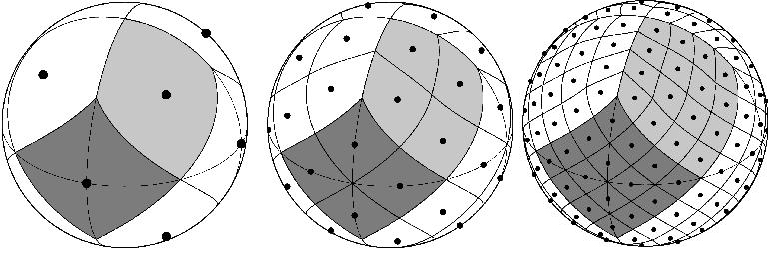
\includegraphics[width=0.95\textwidth]{figures/healpix-3layers.jpg}
\caption{3 smaller sclales of the healpix sampling.}
\label{fig:healpix_sampling}
\end{figure}

\section{Related work}
\label{sec:related}



\subsection{Spherical convolutions} 
The major challenge to generalize CNN to a
spherical domain is to generalize convolution. In the context of CNN, we found
two particular approaches to address this issue.

The first approach, leveraging the continuous spherical convolution, has been
proposed in~\cite{cohen2017convolutional,cohen2018spherical}. These
contributions propose to use a convolution that is rotational equivariant on the
sphere, i.e. a rotation of the input implies the same rotation of the output.
The convolution is performed by a spherical Fourier transform (i.e. a projection
on the spherical harmonics), a  multiplication in the spectral domain and an
inverse spherical Fourier tranform. Hence the main computational cost of a
convolution comes from the two Fourier transforms. Fortunately, the Fourier
transform can be accelerated for special samplings set (theoretically including
HealPix). The main advantage of this approach is that it provides a
mathematically well defined rotational equivariant network. Nevertheless, even
with these Fourier transform acceleration, the convolutions remain expensive in
comparison to a traditional 2-dimensional convolution, limiting the practical use of this
approach. While a comparison is theoretically possible, the experiments
of~\cite{cohen2018spherical} are done using the geodesic grid sampling set and
do not provide any code for the Healpix one. Hence, a practical comparison is
not possible.

A second direction has been followed in~\cite{boomsma2017spherical}. The idea is
to use the traditional 2-dimensional convolution on an irregular grid defined on the
sphere. In the paper, two grids are used: the geodesic grid and the “cubed
sphere” grid defined by Ronchi et. al~\cite{ronchi1996cubed}. Because this
approach is based on the traditional 2-dimensional convolution, it is very likely to be the
most efficient one. However, it suffers that it can only be used using very
specific grid sampling sets which are NOT including HealPix. Furthermore, the
grid requirement makes it impossible for the convolution to capture the
spherical properties of the domain, i.e. the "cubed sphere” sampling is by
definition adapted to a cube and not to a sphere. \nati{Michael: Under some very
specific hypothesis, this second approach is a particular case of our method,
i.e. 1) our method with a stupid sampling, 2) assumption that graph convolution
on a grid == 2d convolution. Do you think we should mention that? I think we
should not.}

In an attempt to get the best of the two approaches, we follow a third
direction. We use a graph to adapt to the particular structure of the sphere.
While the convolution remains efficient, it still captures well the spherical
structure and is particularly adapted to the HealPix sampling.

\subsection{Convolutions on graphs}
\assign{Michaël}

\todo{other approaches? GNNs, Kipf first order approx, message passing}

Previous work: [Bruna] which needed the full eigendecomposition of the Laplacian, costing $O(n^3)$ operations.

In this work, we are using the graph CNN formulation introduced in~\cite{defferrard2016convolutional}.

Spatial definitions of graph convolutions, e.g. [Niepert] needs to define an orientation in order to match the edges with the filters. Most often the orientation is not given by the application, and one has to define it (for example by ordering by degree or any other measure, or by using a graph coloring). There is no good default good orientation on general graphs and the choice of an orientation is highly application dependent.

\todo{Cool to have a global illustration of the network (CNN like)}

\subsection{Convolutions on manifolds}

Related to this, convolutional neural networks have been defined on manifolds and have achieved impressive results on shapes [Bronstein]. They however too depend on an orientation, which spheres do not possess.

\subsection{Convolutions on point clouds?}

PointNet and co. Related but we are loosing the structure. Also coarsening.

\section{Method}
% \begin{itemize}
% 	\item We build a graph using the healpix sampling
% 	\item Define Fourier transform and show that the harmonics are visually close to the spherical harmonics
% 	\item Define spherical convolution using the graph Fourier transform and show heat diffusion example
% 	\item Show the limits of the approach and explain why we cannot have a perfect spherical convolution with this technique
% \end{itemize}

The gist of our method is to define the convolution on a sphere using a graph.
The graph is here seen as a discrete approximation of the sphere $S^2$, a
2-dimensional manifold embedded in $\mathbb{R}^3$.

As presented in~\cite{cohen2018spherical}, the most mathematical approach to
extend the convolution on a sphere is to use a spherical Fourier transform. The
convolution is then simply defined as the product in the spectral domain. This
approach requires one Fourier and one inverse Fourier transform per convolution
which remain, even with accelerated algorithms, expensive. For 2-dimensional
images, an efficient convolution can be achieved when the convolution kernel is
localized (for example a 5x5 pixel patch) by doing the computation directly in
the signal domain. Unfortunately, this approach cannot be directly extended to
the spherical case. Hence, the main idea of this contribution is to leverage
graph signal processing~\cite{shuman2013emerging} to define a spherical
convolution that can be computed directly in the signal domain.

\subsection{Graph creation}
In the classical 2-dimenstional convolution, each pixel is connected with the
same weight to its 4 closest neighbors. We use a weighted undirected graph to
generalize this idea to the ubiquitous HealPix
sampling~\citep{gorski2005healpix}.  Each pixel is represented by a node
(vertex) connected to his $8$ or $7$ closest neighbors.\footnote{For some
pixels, the $8^{th}$ nearest neighbor is not well defined.} Given the set of
nearest neighbors, we define the weight matrix $W$ using the following scheme
\begin{equation}
W[i,j]=\begin{cases}
e^{-\frac{\|x_i-x_j\|_2^2}{\sigma^2}} & \text{if pixels $i$ and $j$ are connected, and}\\
0 & \text{otherwise.}\\
\end{cases}
\end{equation}
Here $x_i$ is a 3-dimensional vector encoding the coordinate of the pixels $i$
on the sphere and $\sigma$ is the mean of $\|x_i-x_j\|_2$ over all connected
pixels $i$ and $j$. This weighting scheme is important as the distances between
pixels varries du to the small sampling irregularities. Some of the
irregularities have been highlighted in the graph displayed in
Figure~\ref{fig:healpix_graph_4}.

These small irregularities are important and affect slightly the degree of a 
node (or a pixel), defined as $d_i =\sum_j W[i,j]$. 

\begin{figure}[!ht]
\centering
% 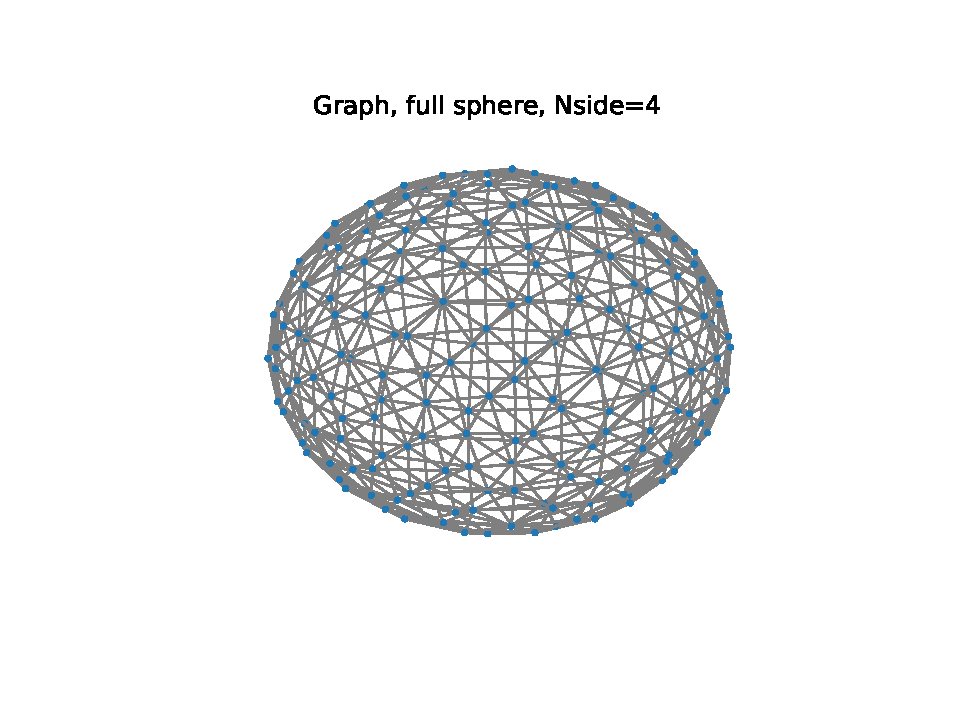
\includegraphics[width=0.45\textwidth]{figures/healpix_graph_4.pdf}
\vspace{-0.5cm}
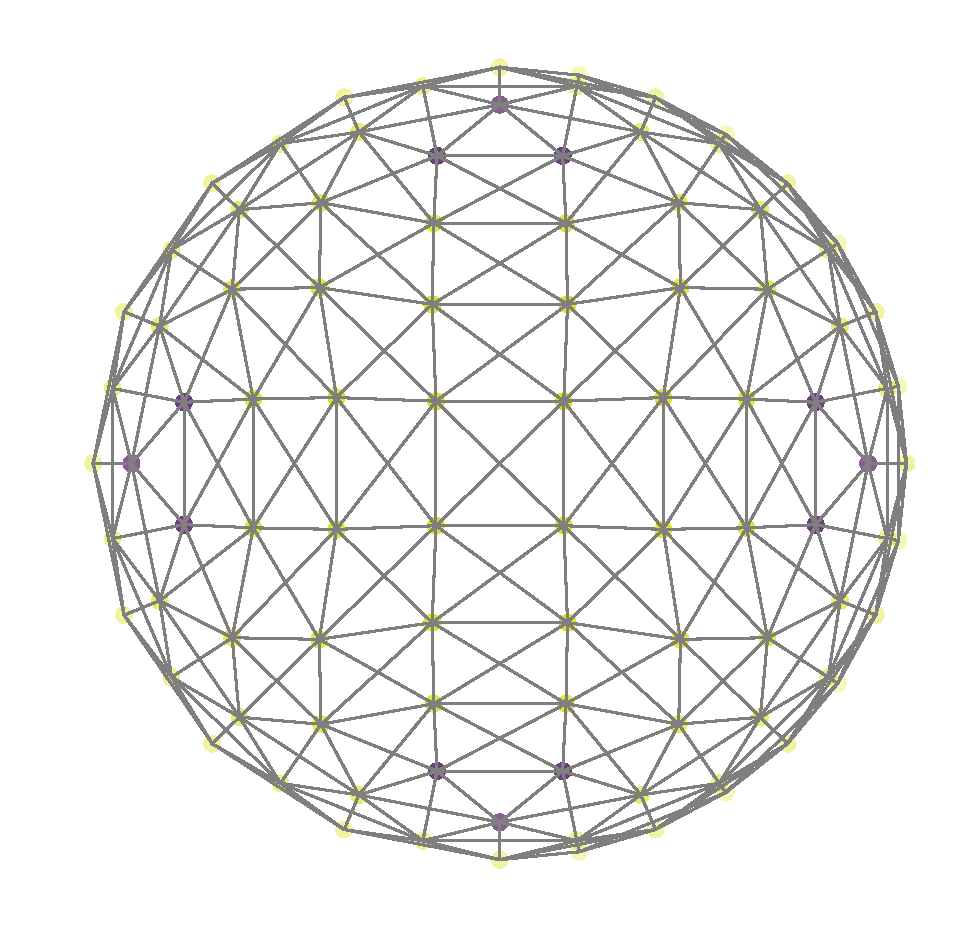
\includegraphics[width=0.45\textwidth]{figures/half_graph_4.pdf}
\vspace{-0.5cm}
\caption{
% Left: Healpix graph for the full sphere using a nside parameter of $4$. 
Top view of a Healpix graph for half the sphere using a nside parameter of $4$.}
\label{fig:healpix_graph_4}
\end{figure}

\subsection{Graph Fourier basis and spherical harmonics}
\todo{Add a few extra references}

Because of the irregular sampling, there is no obvious way to define convolution
directly from the pixel values. Hence we first define a Fourier transform on the
graph.

Following~\cite{shuman2013emerging}, the graph normalized graph Laplacian
defined as $\L = \I - \D^{-1/2} \W \D^{-1/2}$ is a second order differential operator
that can be used to define the graph Fourier basis. Here $D$ is the diagonal
matrix where $\D_{ii}=\b{d}_i$. By construction the Laplacian is symetric postive
semi-definite and hence can be decomposed as $\L=\U \bLambda \U^*$, where $U$ is an
orthonormal matrix of eigenvectors and $\bLambda$, the diagonal matrix of
eigenvalues. The graph Fourier basis is defined as the Laplacian eigenvectors.
The graph Fourier transform of $f$ is simply its projection on $U$ given by 
$\hat{\b{f}}=\U^*\b{f}$. Similarly the inverse graph Fourier transform reads $\b{f}=\U\hat{\b{f}}$.
Note that instead of frequencies, the Fourier modes are crescently ordered with
respect of the Laplacian eigenvalues $\bLambda$. In a sense, the Laplacian
eigenvalues correspond to the squared frequencies. 

\begin{figure}[!ht]
\centering
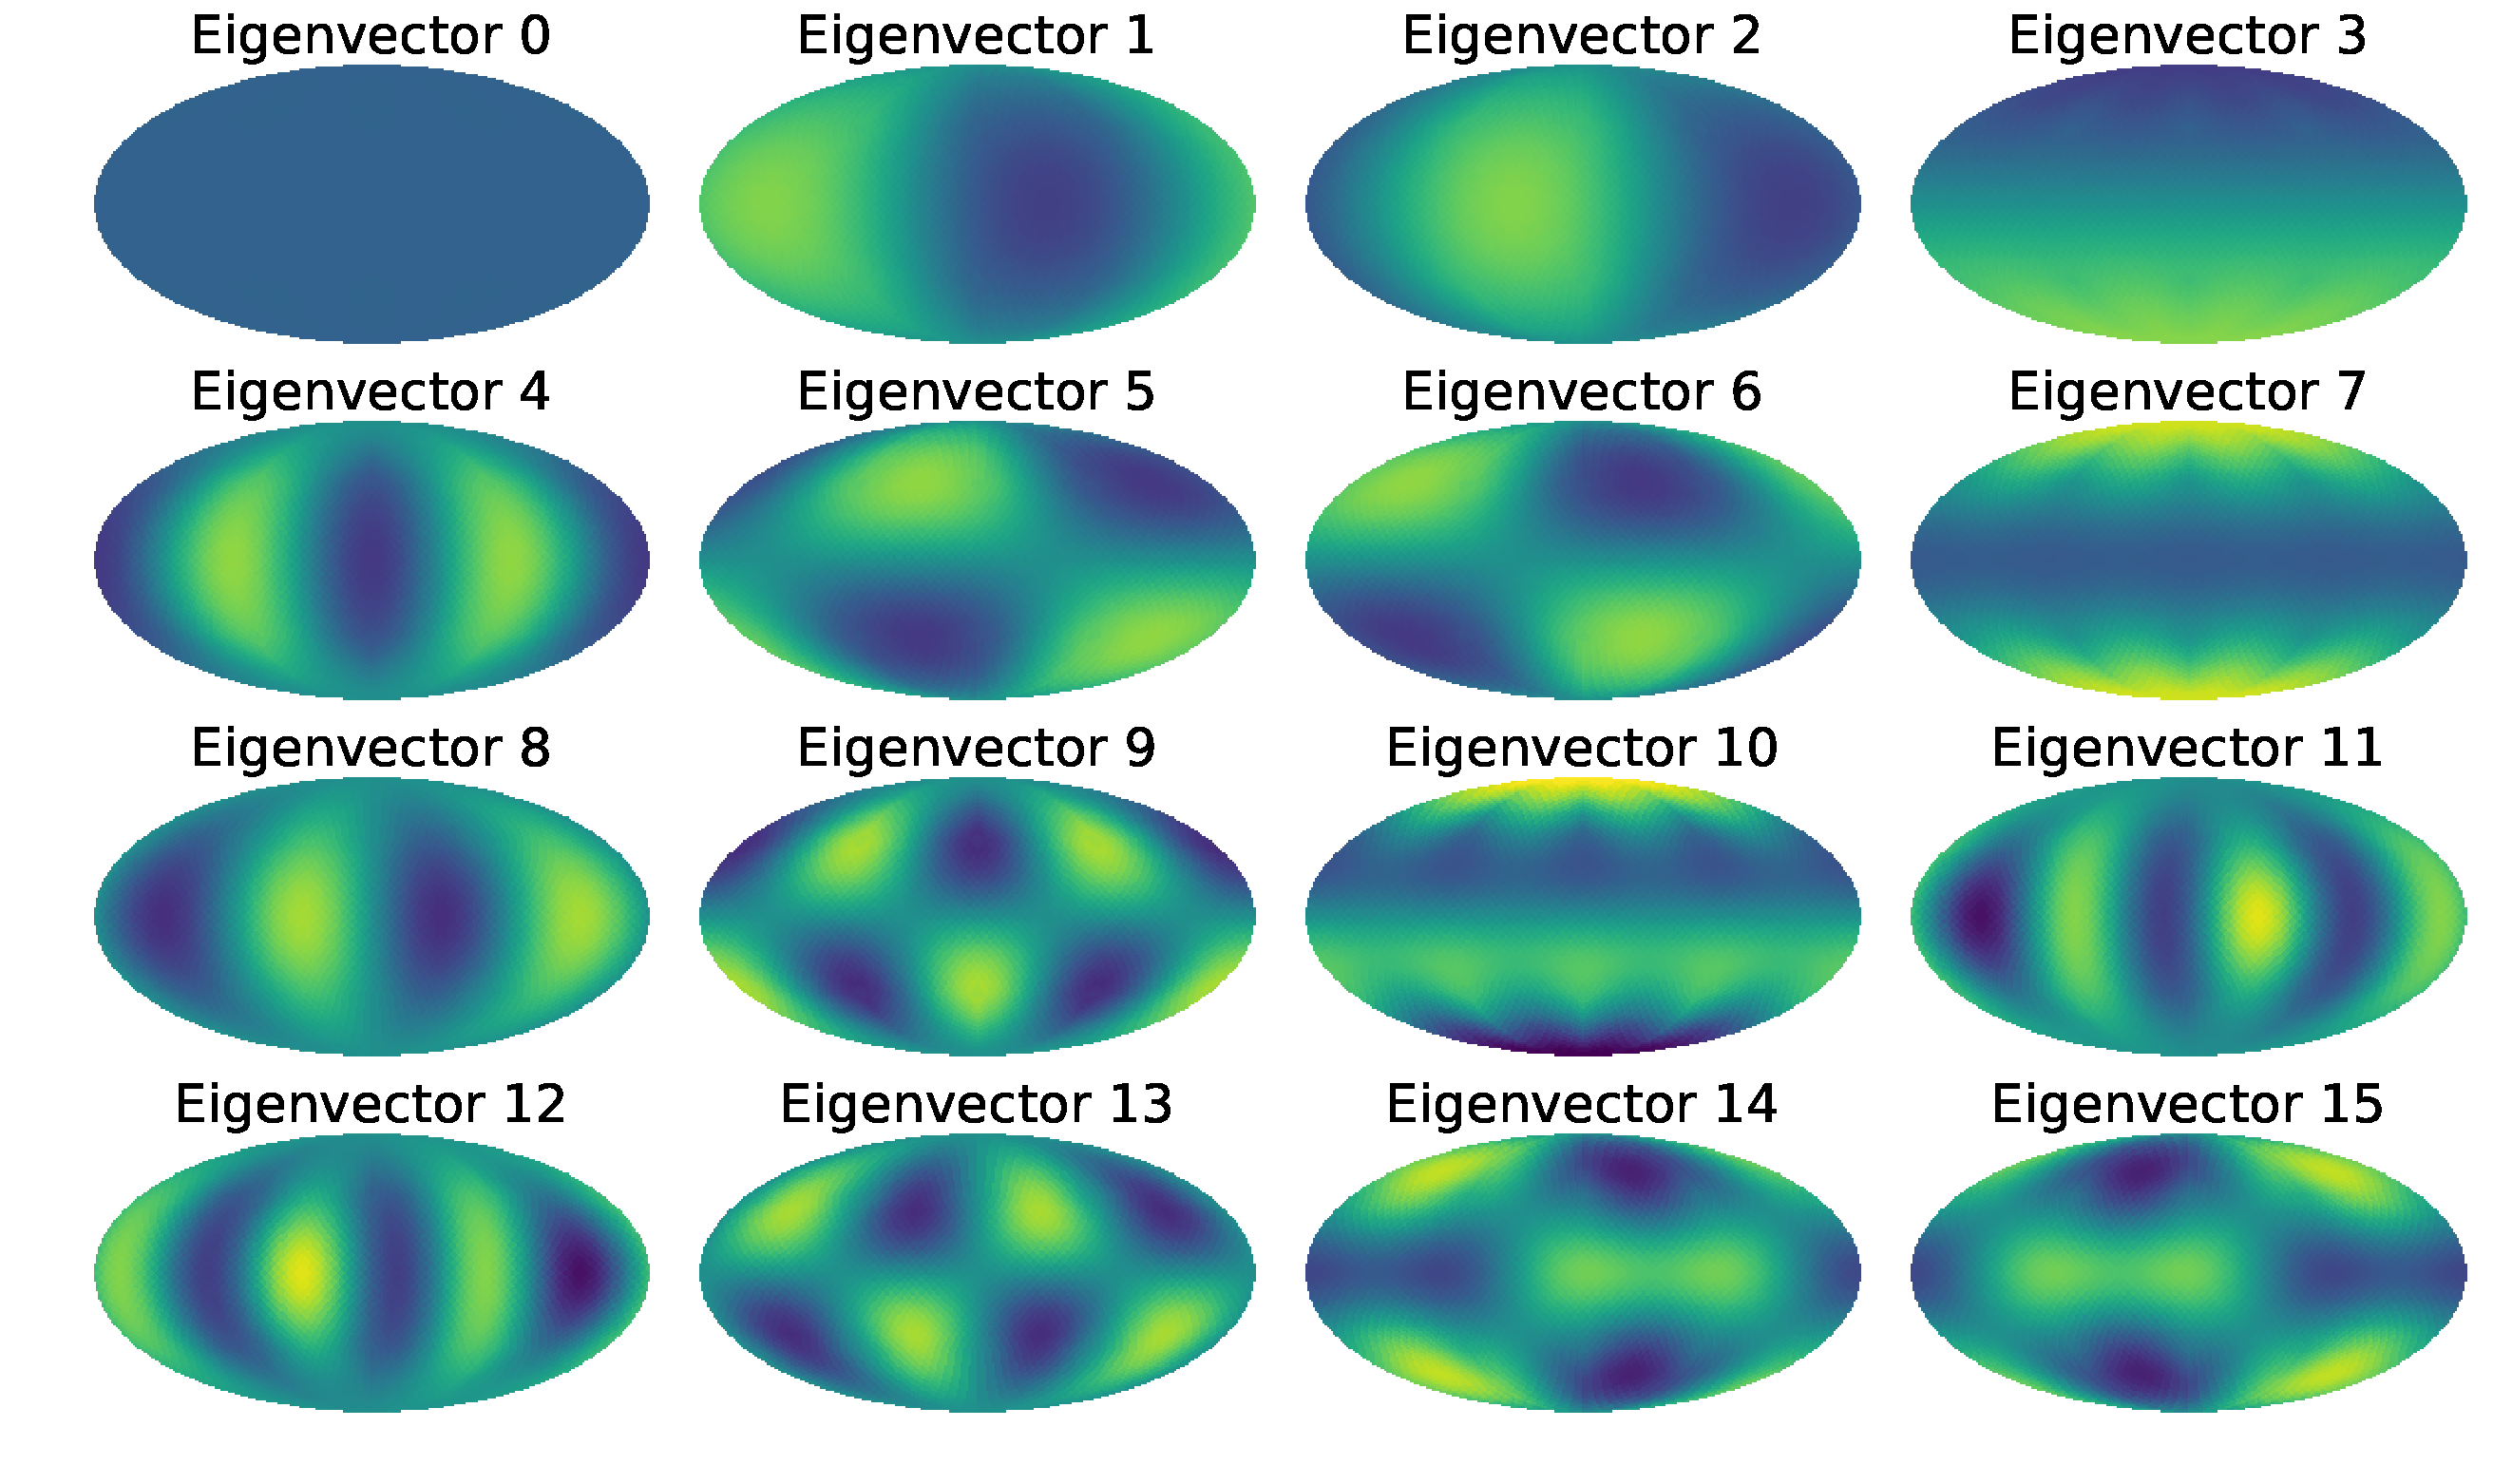
\includegraphics[width=0.95\textwidth]{figures/eigenvectors.pdf}
\caption{12 first graph Fourier eigenvectors.}
\label{fig:graph_harmonics}
\end{figure}

As shown in Figure~\ref{fig:graph_harmonics}, it turns out that using the graph
construction described above, the graph Fourier harmonics ressembles the
classical spherical harmonics giving us an indication that the graph is able to
capture the spherical properties of the HealPix sampling.

\subsection{Convolutions on graphs}
\assign{Nathanaël, Michaël} \todo{Add a few extra references}

Graph convolution is defined by generalizing the concept that convolution is a
multiplication in the spectral domain. Given a convolution kernel 
$h:\mathbb{R}_+\rightarrow\mathbb{R}$, the convolution of a signal $\b{f}$ 
is defined as
\begin{equation} \label{def:graph_convolution}
h(L)\b{f} = \U h(\bLambda) \U^* \b{f},
\end{equation}
where $h(\bLambda)$ is a diagonal matrix where $h(\bLambda)_{ii}=h(\bLambda_{ii})$.
Equation~\ref{def:graph_convolution} contains three parts: a) $\U^* \b{f}$, the 
Fourier transform of $\b{f}$; b) $h(\bLambda)$ the multiplication with the Fourier 
kernel $h(\blambda)$; and c) $\U$ the inverse Fourier transform.

The major difference with classical convolution is that the convolution kernel
$h$ cannot be thought as $n \times n$ pattern, but is a continuous function
applied to the graph eigenvalues $\bLambda$. For visualization puposes, one can
look at effect of the convolution on a dirac, i.e. one column of the matrix
$h(\L)$. \nati{However, due to the non regularity of the graph (i.e. the fact
that there is not perfect sampling on the sphere), this visualization will
differ from one node to another. In the specific case of the full sphere, these
difference are negligible in most of the cases. When considering only subpart of
the sphere, one will observe important border effects.}

\paragraph{Example: heat diffusion}
Let us consider the heat diffusion problem 
\begin{equation} \label{eq:heat_equation}
\L \b{f}(t) = \tau \partial_t \b{f}(t),
\end{equation}
where $\b{f}(t): \mathbb{R}_+ \rightarrow \mathbb{R}^N$. Given the initial condition 
$\b{f}(0)$, the solution of~\ref{eq:heat_equation} can be expressed as
\begin{equation}
\b{f}(t) = e^{-\L \tau t} \b{f}(0) = \U e^{-\bLambda t \tau} \U^* \g{f}(0) = K_t(\L) \b{f}(0), 
\end{equation}
which is a convolution of the signal $\b{f}(0)$ with the kernel $K_t(x)=e^{-\tau
t x}$. Here the kernel $K_t$ is applied to the graph eigenvalues $\bLambda$ that
correspond to the squared frequencies and hence $K_t$ can be considered a
Gaussian kernel. In Figure~\ref{fig:gaussian_filters_comparizon} top, we show
the effect of the convolution by diffusing a unit of heat for $\tau=1$ and various 
time $t$. In  Figure~\ref{fig:gaussian_filters_visualization} of
Appendix~\ref{app:filter_visualization}, we show different visualizaton of the
convolution kernel $K_t$. We also compare the graph convolution with the
spherical symmetric Gaussian smoothing
(Figure~\ref{fig:gaussian_filters_comparizon} bottom) and observe that both
techniques lead to similar results. While the graph convolution is different
from a true spherical convolution, it can, providing the correct
parametrization, well approximate it.

\begin{figure}[!ht]
\centering
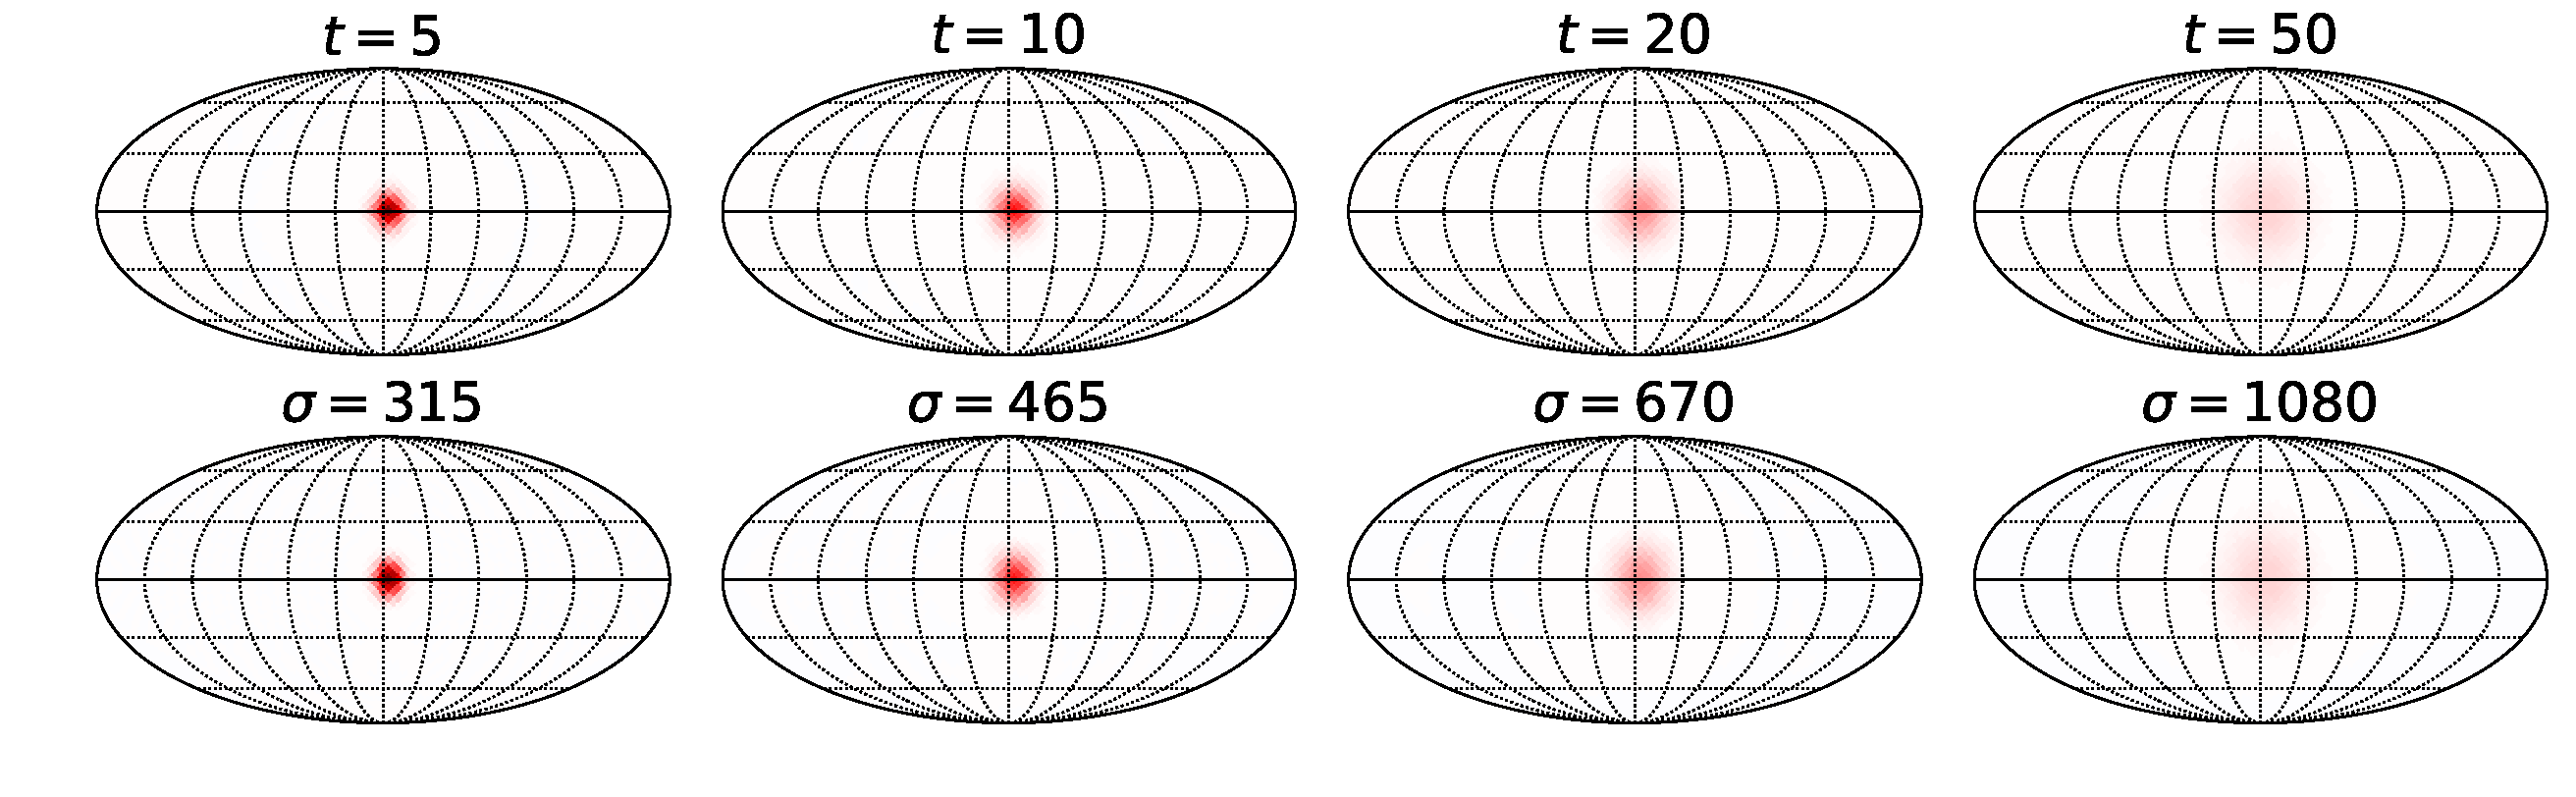
\includegraphics[width=0.95\textwidth]{figures/gaussian_filters_sphere.pdf}
\caption{Convolution comparizon (Nside=16). 
Top: Diffusion of a unit of heat for different time $t$ using the graph. 
Bottom: spherical symmetric Gaussian smoothing for different $\sigma$ (arcmin). 
Relative difference between graph convolution and spherical smoothing: $10.4$\%, $5.7$\%, $4.8$\%, $3.8$\% }
\label{fig:gaussian_filters_comparizon}
\end{figure}

It is another sign that the constructed graph is able to capture the spherical
structure of the healpix sampling. Furthemore, in some application, where the
exactitude of the convolution is not requirement, such as de-noising, it means
that we could use graph convolution instead. Depending on the convolution kernel
this may reveal much more efficient. In the case of a neural network, the fact
that both convolution are not identical is not very relevant since the network
will adapt the convolution at use.

\subsection{Efficient convolutions}
\assign{Michaël}
With the Fourier basis. Because we don't have an FFT, that costs $O(n^3)$ for the eigendecomposition, plus $O(n^2)$ for the transform (to be done for each forward and backward pass).
\begin{itemize}
	\item We need efficient convolution, hence the Chebysheff trick
	\item Explain the different between a polynomial filter convolution and a traditional patch restricted convolution
	\item Define spherical CNN using graph CNN
\end{itemize}


\subsection{Coarsening}
The HealPix sampling present the advantage to have a natural corsening method
based on its construction. Each nside level divides each pixel into 4 subpixels.
We define the pooling process as the inverse operation grouping the 4 subpixels.
Figure~\ref{fig:pooling} illustrates the process.
\begin{figure}[!ht]
\centering
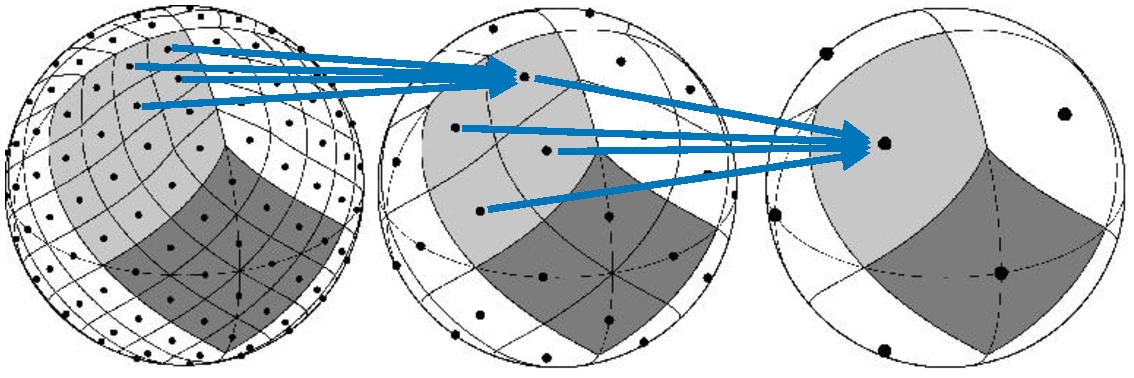
\includegraphics[width=0.95\textwidth]{figures/pooling.pdf}
\caption{Pooling illustration for 2 levels using some part of the the mollview projection. 
The final patch represent 1/12 of the sphere.}
\label{fig:pooling}
\end{figure}


\section{Experiments}

What do we want to show? The graph CNN is able to discriminate ??? using higher order statistics.

\subsection{Data}
\assign{Tomek}

Our data comes from a simulation with software ??? using the following parameters ???. All the data to reproduce our experiments are available online.\footnote{\url{https://doi.org/10.5281/zenodo.????} \todo{correct DOI}}

\begin{figure}[!ht]
\centering
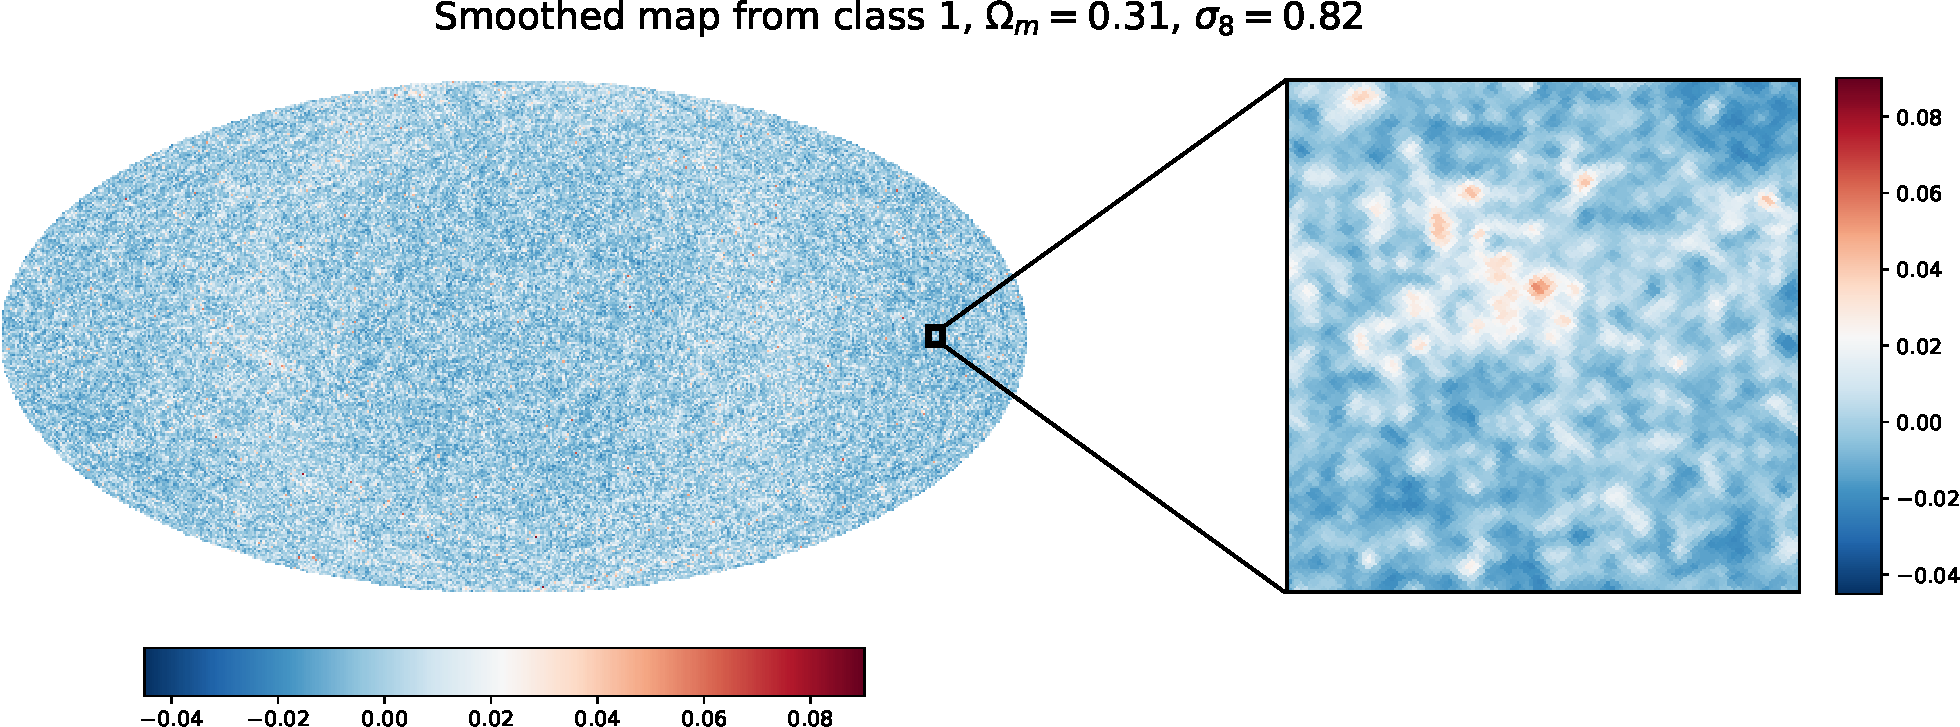
\includegraphics[width=0.45\textwidth]{figures/smooth_map_class_1.pdf}
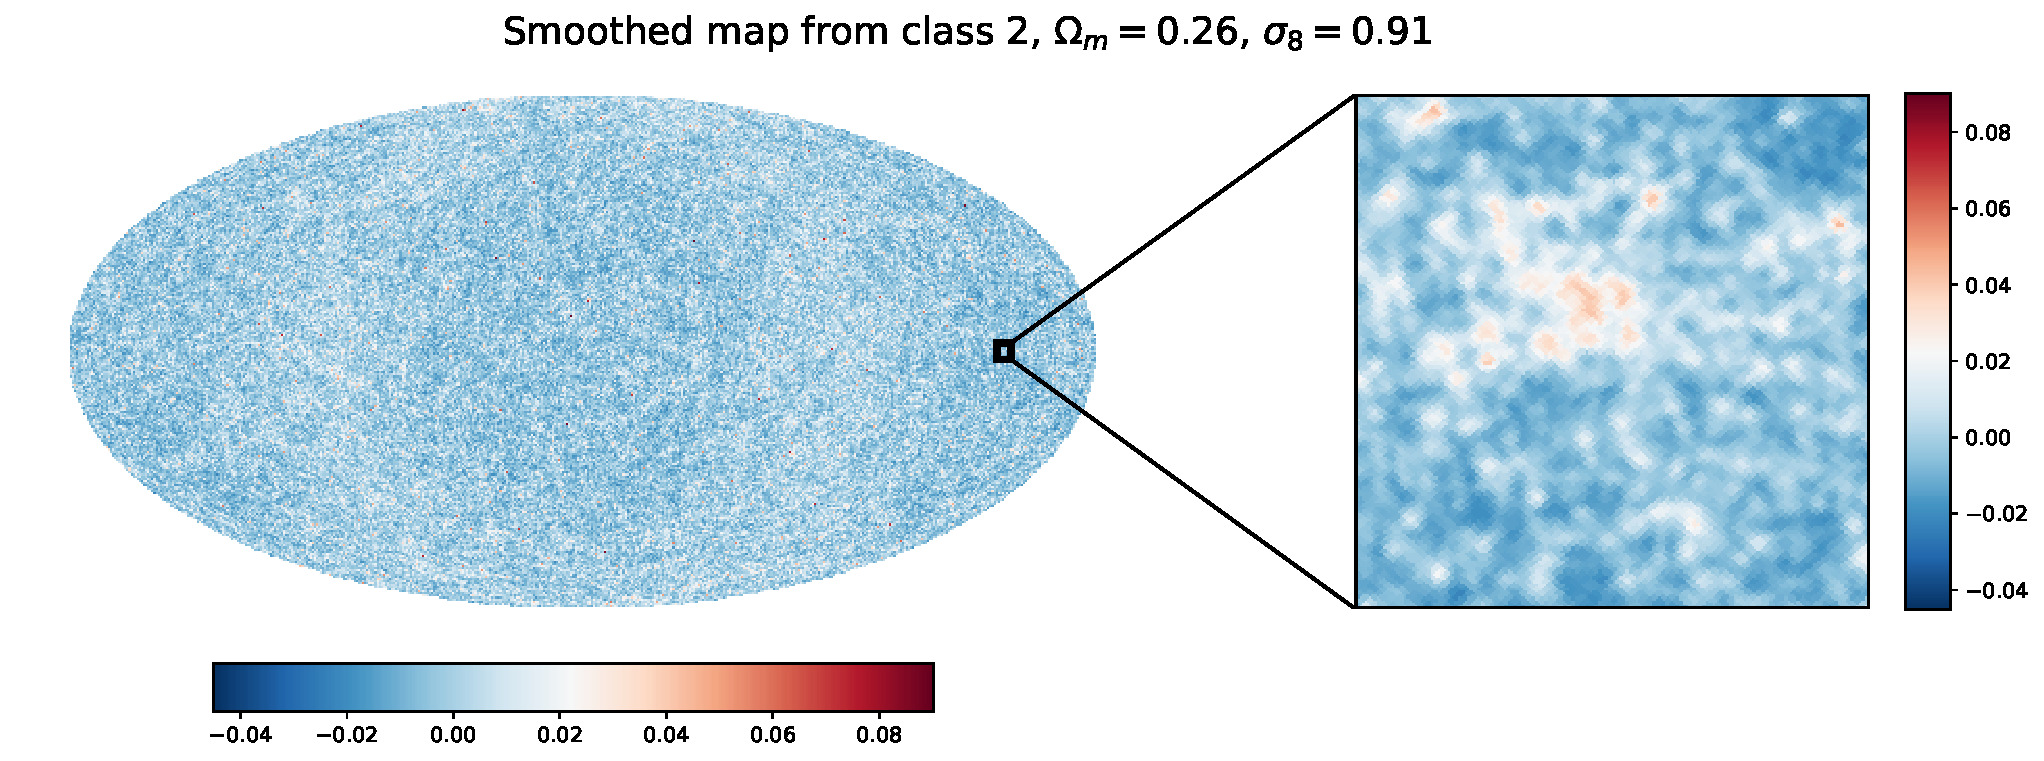
\includegraphics[width=0.45\textwidth]{figures/smooth_map_class_2.pdf}
\caption{One sample of each class }
\label{fig:map_sample}
\end{figure}

\begin{figure}[!ht]
\centering
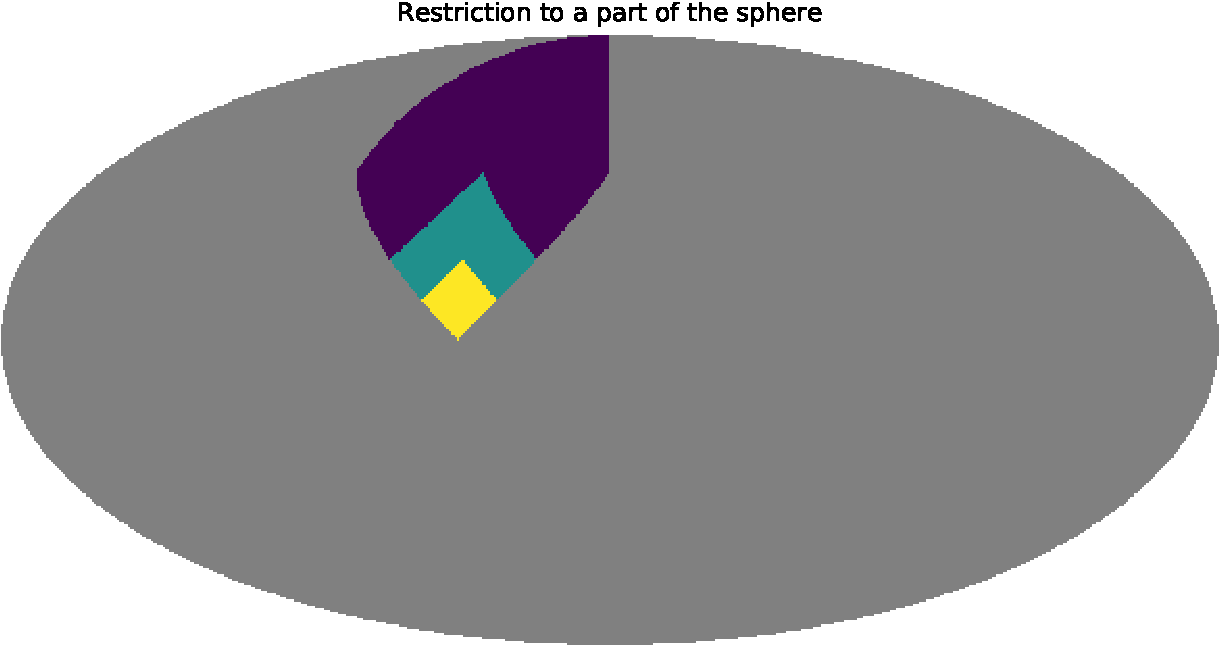
\includegraphics[width=0.45\textwidth]{figures/part_sphere.pdf}
\caption{3 subparts of the sphere with different sizes. Blue: order 1. Green: order 2. Yellow: order 3.}
\label{fig:subpart_sphere}
\end{figure}

\subsection{Results}

\begin{figure}[!ht]
\centering
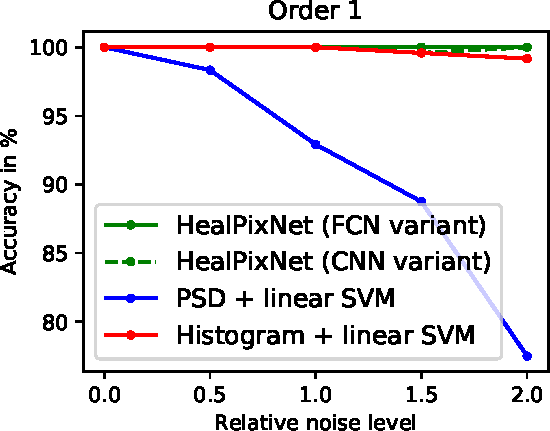
\includegraphics[width=0.32\textwidth]{figures/result_order1.pdf}
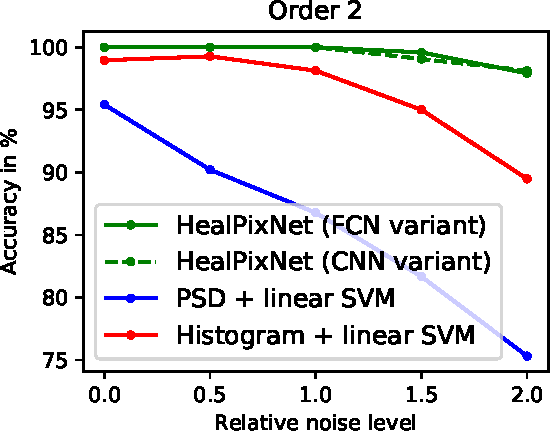
\includegraphics[width=0.32\textwidth]{figures/result_order2.pdf}
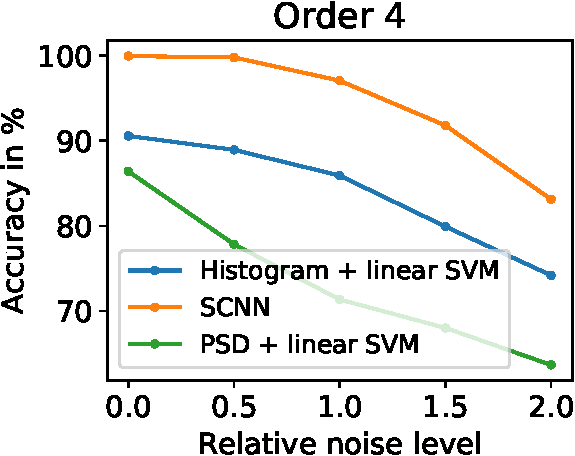
\includegraphics[width=0.32\textwidth]{figures/result_order4.pdf}
\caption{Classification errors for the 3 different problems.}
\label{fig:results}
\end{figure}

\assign{Nathanaël, Tomek}

\begin{itemize}
	\item With the entire sphere / different PSD (The PSD features + linear SVM is equivalently good)
	\item Without the entire sphere / same PSD (1 sample: the histogram features + kernelized SVM is equivalently good)
	\item ??
\end{itemize}


Figure: Result curves 

Figure: Filters 1D and Gnonomic

\subsection{Interpretation}
\assign{Nathanaël, Tomek, Michaël}

Show the learned filters and feature maps and try to interpret them.

\section{Conclusion}
\assign{Nathanaël, Tomek, Michaël}

\section*{Thanks}

%% The Appendices part is started with the command \appendix;
%% appendix sections are then done as normal sections
\appendix

\section{Filter visualization}
\label{app:filter_visualization}

In Figure~\ref{fig:gaussian_filters_visualization}, we present three different
ways to plot the graph convolution kernel $K_t(x)=e^{-\tau t x}$.  First, it can
be ploted in the graph spectral domain. In this case, we simply evaluate $K_t$
at the graph eigenvalues $\text{diag}(\bLambda)$. Second, we can convolve a
delta on the sphere and plot a gnomonic view of the results. Third, since we are
working on the sphere, we can only plot the section of the convoluted delta. In
Figure~\ref{fig:index_section}, we display the selected indexes for the section
plotting. Note that, because of the small irregularities in the HealPix
sampling, the second and the third methods are likely to change depending on the
chosen delta.

\begin{figure}[!ht]
\centering
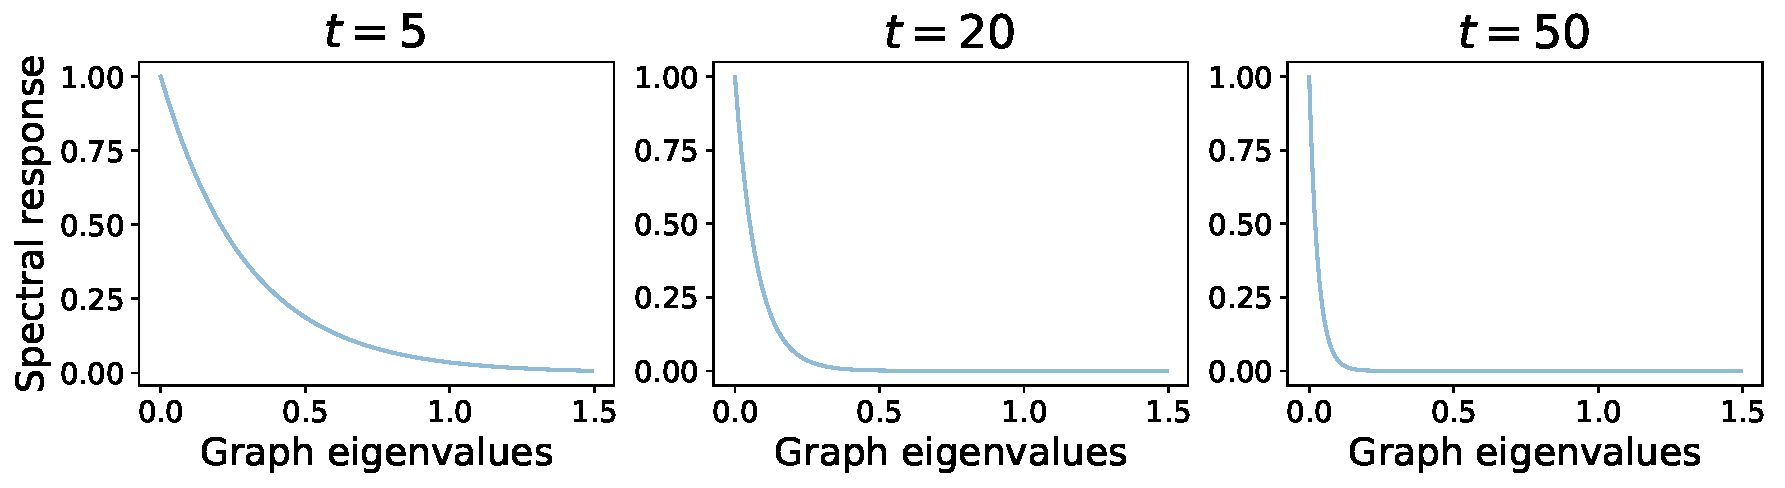
\includegraphics[width=0.95\textwidth]{figures/gaussian_filters_spectral.pdf}
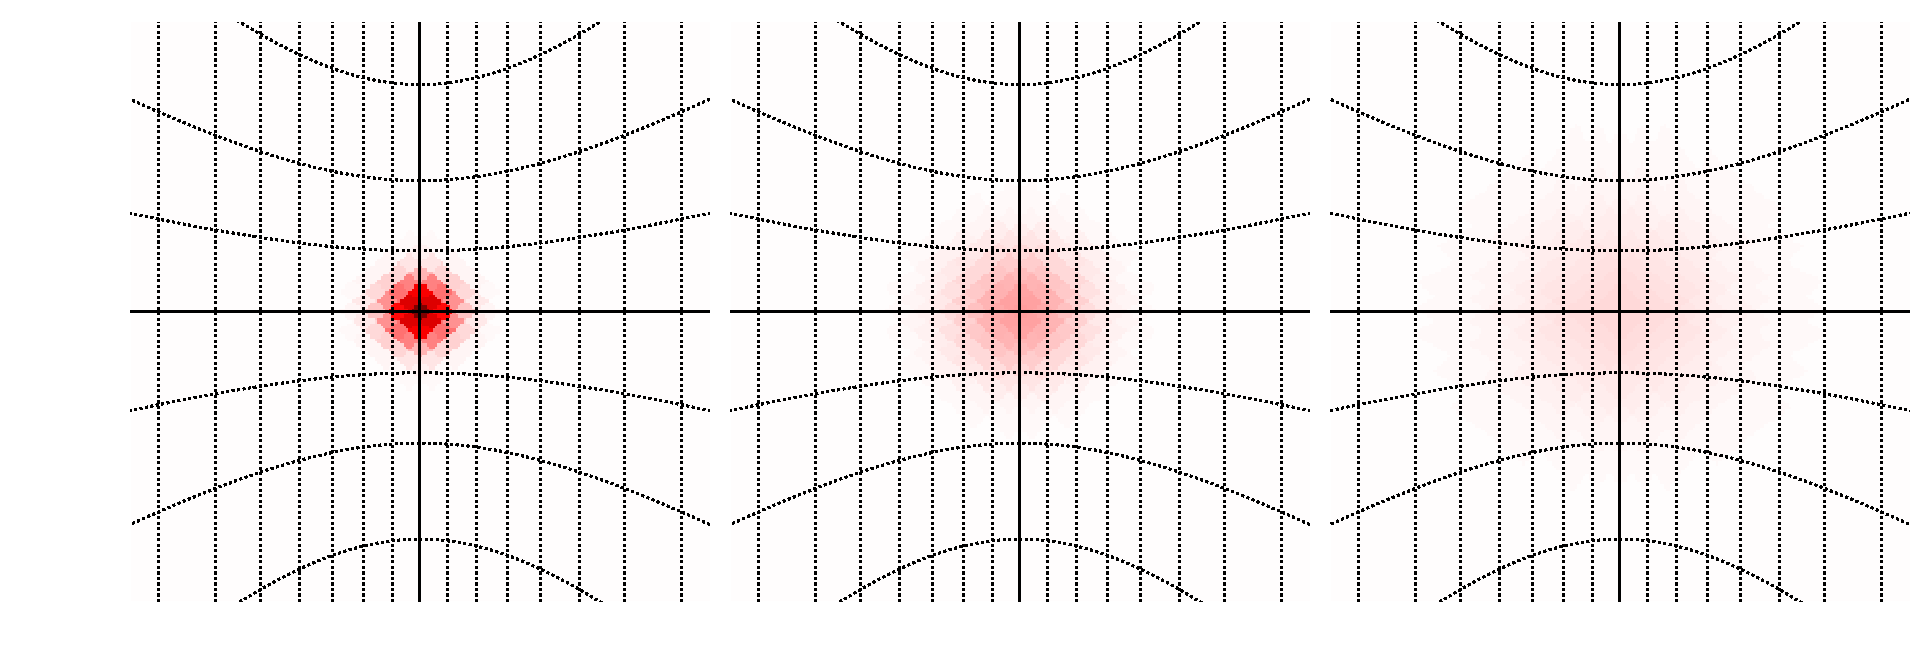
\includegraphics[width=0.95\textwidth]{figures/gaussian_filters_gnomonic.pdf}
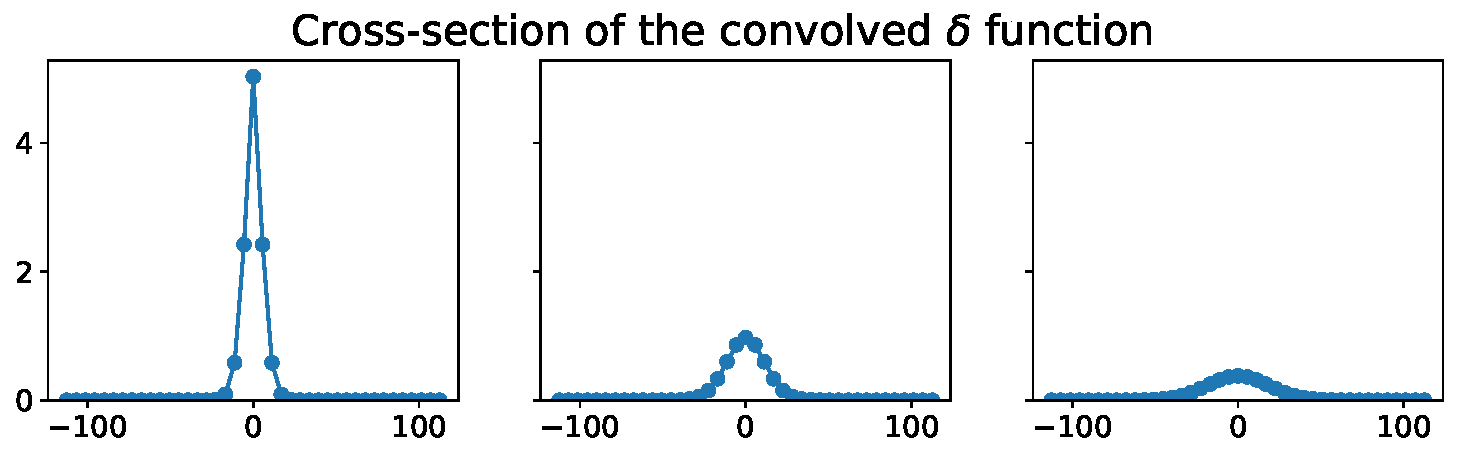
\includegraphics[width=0.95\textwidth]{figures/gaussian_filters_section.pdf}
\caption{3 different visualizations of the convolution kernel $K_t(x)=e^{-\tau t x}$.  
Top: graph spectral domain. 
Middle: gnomonic projection.
Bottom: section plot.}
\label{fig:gaussian_filters_visualization}
\end{figure}

\begin{figure}[!ht]
\centering
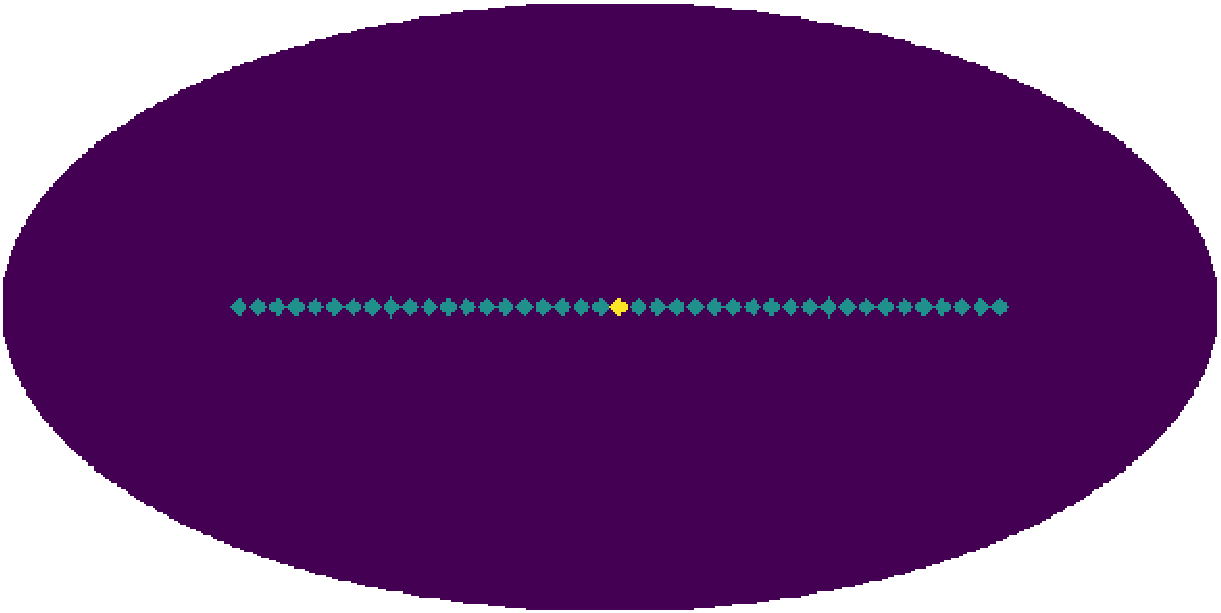
\includegraphics[width=0.45\textwidth]{figures/index_plotting_order20_nside16.pdf}
\caption{Indexes selected for the section ploting of Figure~\ref{fig:gaussian_filters_visualization} middle. The delta was placed on the yellow node.}
\label{fig:index_section}
\end{figure}



%% If you have bibdatabase file and want bibtex to generate the
%% bibitems, please use
%%
\section*{Bibliography}
\bibliographystyle{elsarticle-harv} 
\bibliography{biblio}

\end{document}

\endinput
%%
%% End of file `elsarticle-template-harv.tex'.
